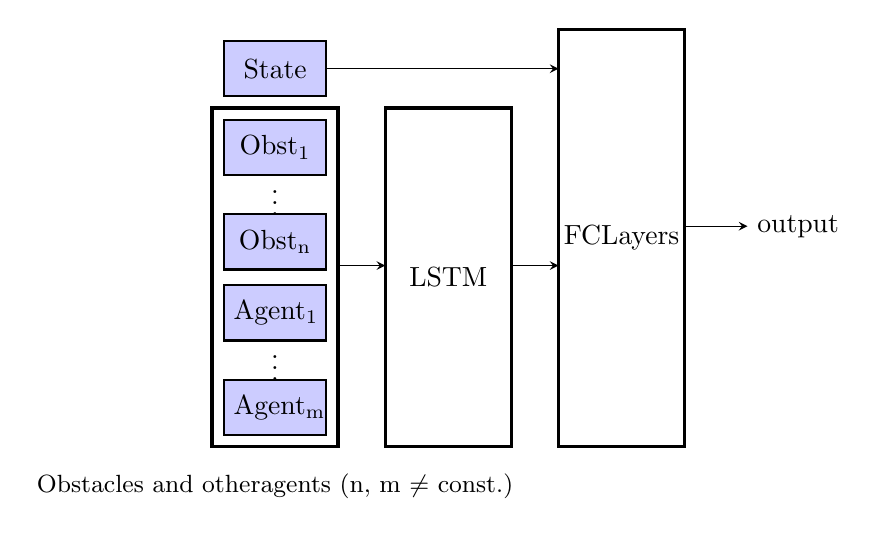
\begin{tikzpicture}
    [block_o/.style = {rectangle, draw=black, thick, width=5em, height=10em},
    block_on/.style = {rectangle, draw=black, fill=white!80!blue, thick, text width=3em,align=center, minimum height=2em}]

    % Agent block
    \draw (-2,3.5) node[block_on] (A) {State};

    % Obstacles block
    \draw[black, very thick] (-2.8,-1.3) rectangle (-1.2,3);
    \draw (-2,-1.8) node[] {\makecell{\small Obstacles and other \\ \small agents (n, m $\neq$ const.)}};
    \draw (-2,2.5) node[block_on] (O1) {Obst\textsubscript{1}};
    \draw (-2,1.9) node[] {\vdots};
    \draw (-2,1.3) node[block_on] (On) {Obst\textsubscript{n}};
    \draw (-2,0.4) node[block_on] (A1) {Agent\textsubscript{1}};
    \draw (-2,-0.2) node[] {\vdots};
    \draw (-2,-0.8) node[block_on] (Am) {Agent\textsubscript{m}};

    % RNN block
    \draw[black, very thick] (-0.6,-1.3) rectangle (1.0,3) node[midway, anchor=center] {\makecell{LSTM}};

    % FC block
    \draw[black, very thick] (1.6,-1.3) rectangle (3.2,4) node[midway, anchor=center] {\makecell{FC \\ Layers}};
    
    % Connections
    \draw[-stealth] (A) -- (1.6,3.5);
    \draw[-stealth] (-1.2, 1) -- (-0.6, 1);
    \draw[-stealth] (1.0, 1) -- (1.6, 1);
    \draw[-stealth] (3.2, 1.5) -- (4.0, 1.5) node[anchor=west] {output};

\end{tikzpicture}